\section{Optimal hedge ratio}\label{sec:optimal-hedge-ratio}

\subsection{Distribution of hedge portfolio}\label{subsec:DHP}
We form a portfolio with two assets, consisting of one unit in the
spot asset and a short position of $h$ units of a futures contract,
for example one Bitcoin and a short position in a CME Bitcoin
futures contract. 
The objective is to minimize the risk of the exposure in the spot. 
Let $R^S$ and $R^F$ be the (discrete) returns of the spot and
futures price. The (discrete) return of the portfolio is\footnote{%
In practice, as the nominal investment in the futures is zero, $R^F$
is understood as the return on the notional amount underlying the
futures contract. In other words, if both the spot price $S_{t-1}$
and the futures price $F_{t-1}$ are 
normalised to $1$, then the portfolio return will be identical to the
portfolio value change $\Delta V = \Delta S - h \Delta F$, where $\Delta S =
S_t-S_{t-1}$, etc.}
\begin{equation*}
R^h = R^S -h R^F.
\end{equation*}
%\natp{\em [I fixed this, please check.] [We need to discuss the
%  footnote. Generally, the portfolio return is $R_p = \sum_{i=1}^n w_i
%  R_i$. With the futures contract, the notional investment in the
%  futures is zero, so the portfolio return is $(S_0 (1+R^S) -h F_0
%  R^F)/S_0-1 = R^S-h R^F$, if $S_0=F_0$.]}

The risk of the hedged portfolio is measured by risk measure functions.
For example, a widely used risk measure is value-at-risk (VaR), which,
at the confidence level $\alpha$,
is derived from the $1-\alpha$ quantile of the return distribution. %  at the confidence level $\alpha$ is
% the absolute value of the $1-\alpha$-quantile of $R^h$, i.e., $\text{VaR}_{1-\alpha} =
% -F_{R^h}^{(-1)}(1-\alpha) = -\inf\{x \in \mathbb{R}: 1-\alpha \leq
% F_{R^h}(x) \}$, where $F_{R^h}$ is the distribution function of
% $R^h$.

If the portfolio intended to reduce the risk of the spot position, then
we call this a hedged portfolio.
An optimal hedge ratio $h^*$ is a parameter that
minimizes the risk of the aforementioned portfolio
\begin{equation*}
h^* = \argmin_h \rho(R^h).
\end{equation*}

Obviously the cdf and pdf of $R^h$ and the risk measure depend on the
joint distribution of $R^S$ and $-hR^F$. However, optimising $h$
according to the joint pdf is unfavourable since one would need to
calibrate it whenever she updates $h$.
Another problem of using the joint pdf is that one lacks the
flexibility to model the margins separately from the dependence
structure. Copulae allow to overcome both of these problems. 

The advantage of using copulae is two-fold.
First, copulae are invariant under strictly
monotone increasing function \citep{schweizer1981nonparametric}, a
property used in Lemma \ref{lemma:copula} below. 
Second, copulae allow us to model the margins and dependence structure 
separately, a result known as Sklar's Theorem \citep{Sklar1959}, which
is given as Theorem \ref{theorem:sklar} below. 
See also \citep{Nelsen1999, joe1997multivariate, McNeil2005} for
Sklar's Theorem and more properties of copulae.

We adapt the definition of a two-dimensional copula from
\citep{Nelsen1999} as follows.

\begin{defi} [Bivariate copula]
  A {\em bivariate copula} is a function $C: [0,1]^2 \mapsto [0,1]$ with following properties:
  \begin{enumerate}
    \item For every $u,v$ in $[0,1]$,
      \[C(u,0)= C(0,v)=0, \]
    \[C(u,1)= u \text{, and}\]
    \[C(1,v)= v;\]
    \item For every $u_1,u_2, v_1, v_2$ in $[0,1]$ such that $u_1 \leq u_2$ and $v_1 \leq v_2$,
    \[C(u_2,v_2)-C(u_2,v_1)-C(u_1, v_2)+C(u_1,v_1) \geq 0.\]
  \end{enumerate}
  \end{defi}

The second property is called 2-non-decreasing.
In other words, a two-dimensional copula is the joint cdf of a two-dimensional random vector
on a unit square with uniform marginals.

The following Theorem, usually known as the Sklar's
Theorem, ensures the existence of copula which “couples” a 
joint distribution function to its univariate margins \citep[Theorem 2.3.3.]{Nelsen1999}.

% \natp{\em [This is not
%   correct. Copulas, as defined above, exist. Sklar's Theorem links
%   copulas to arbitrary joint distributions.]}

\begin{theorem}[Hoeffding-Sklar-Theorem]
  \label{theorem:sklar}
  Let $F$ be a joint distribution function with marginal distributions
  $F_X$ and $F_Y$. Then, there exists a copula $C:[0,1]^2 \mapsto
  [0,1]$ such that, for all $x,y\in \R$,
  \begin{equation}
    \label{eq:4}
    F(x,y)=C\{F_X(x), F_Y(y)\}.
  \end{equation}
  If the margins are continuous, then $C$ is unique; otherwise $C$ is
  unique on the range of the margins.

  Conversely, if $C$ is a copula and $F_X, F_Y$ are univariate
  distribution functions, then the function $F$ defined by (\ref{eq:4})
  is a joint distribution function with margins $F_X, F_Y$.
\end{theorem}

Hence, copula enables hedgers to model the dependence structure between the spot and futures separately from their marginals 
without any restriction imposed by the model assumption marginals.
For example, the marginals of multivariate Gaussian are always Gaussian, but marginals of copula can be any univariate marginals that hedgers flavour. 
Since we want to focus on the effects of how dependence structure shapes hedging effectiveness, copula allows us to
make minimal model assumption on the marginals by deploying kernel density estimators with different bandwidths for the spot and futures. 

Regarding the theory behind copula, many basic results can be traced back to early
works of Wassily Hoeffding \citep{hoedffding1940, hoedffding1941}. 
The works aimed to derive a measure of relationship of variables,
which is invariant under change of scale. 
See also \citet{hoeffding2012collected} for English translations of
the original papers written in German. 

Another feature of copula that is important for hedgers is shown below. 

\begin{lemma}
  \label{lemma:copula}
  Let $h>0$ and let $X$ and $Y$ be continuous random variables. Then,
  the joint distribution of the portfolio positions 
  can be expressed via the joint distribution of the securities as
  follows:
  \begin{align}
  C_{X, hY}\left(F_X(s),F_{hY}(t)\right) = C_{X,
    Y}\left(F_X(s),F_{Y}(t/h)\right), \quad s,t\in \R.
    \end{align}
  \end{lemma}

\begin{proof}
  Since copulae are invariant under strictly monotone increasing
  function \citet[Theorem 3 (i)]{schweizer1981nonparametric} or
  \citet[Theorem 2.4.3]{Nelsen1999}, 
  \begin{equation*}
    C_{X, hY}\left(F_X(s),F_{hY}(t)\right) = C_{X, Y}\left(F_X(s),F_{hY}(t)\right).
    \end{equation*}
Re-writing the second argument of the copula gives
\begin{equation*}
  F_{hY}(t) = \mathbb{P}(hY \leq t)
  = \mathbb{P}(Y \leq t/h)
  = F_Y(t/h).
\end{equation*}
\end{proof}

%The optimal hedge ratio is $h^\ast = \argmin_h \rho(Z)$, that is the best ratio that can minimize the risk of a hedged portfolio measured in terms of $\rho$ .

Lemma \ref{lemma:copula} describes the fact that copula is invariance under linear transformation.
That means rescaling one random variable does not change the dependence structure captured by copula. 
Searching of optimal hedge ratio (numerically) requires frequent updates of the size of $h$,
but with copula, the search does not require any recalibration.
Taking advantage of Lemma \ref{lemma:copula}, \citet{barbi2014copula}
introduce the distribution of linear combinations of random variables
using copulae. 
We slightly edit their Corollary 2.1 of their work and yield the 
following correct expression of the distribution. 

\begin{proposition}
  \label{prop:dfrh}
  Let $X$ and $Y$ be two real-valued continuous random
  variables on a
  probability space $(\Omega, \F, \p)$ with
  absolutely continuous copula $C_{X, Y}$ and marginal distribution functions $F_{X}$
  and $F_{Y}$. Then, the distribution function of $Z=X-hY$, $h >0$,  is given by
  \begin{equation}
    \label{eq:3}
    F_{Z}(z) = 1- \int^1_0 D_1 C_{X, Y}
    \left[ u, F_{Y} \left\{ \frac{F^{(-1)}_{X}(u)-z}{h} \right\}
    \right]\, d u,   
  \end{equation}
  where, $F^{(-1)}$ denotes the inverse of $F$, i.e., the quantile
function.
\end{proposition}
Here, $D_1 C(u,v)=\displaystyle \frac{\partial}{\partial u}
C(u,v)$ and, see e.g.\ Equation (5.15) of \citet{McNeil2005},
\begin{equation}
  \label{eq:1}
  D_1 C_{X,Y}\{F_X(x), F_Y(y)\} = \p(Y\leq y|X=x).
\end{equation}
\begin{proof}
  Using the identity (\ref{eq:1}) gives
  \begin{align*}
    F_{Z}(z) &= \p(X - h Y\leq z) %
                 = \E\left\{\p\left(Y\geq \frac{X-z}{h}\Big|
                 X\right)\right\}\\[10pt]
               &= 1-\E\left\{\p\left(Y\leq \frac{X-z}{h}\Big|
                 X\right)\right\}% \\[10pt]
               = 1- \int_0^1 D_1 C_{X, Y}\left[u,
                 F_{Y}\left\{\frac{F^{(-1)}_{X}(u) -
                 z}{h}\right\}\right]\, d u.
  \end{align*}
  \end{proof}

%In addition to~\cite{barbi2014copula} we propose a more handy
%expression for the pdf of $Z$.
%\natp{\em [Please double-check the ``+'' signs in the second equation.]}\ \francis{ \em [the + sign is correct.]}

\begin{corollary} The pdf of $Z$ can be written as
  \begin{align}
  f_{Z}(z) &= h^{-1}\int_0^1 c_{X, Y} \left[
  F_{Y}\left\{\frac{F^{(-1)}_{X}(u)-z}{h}\right\}, u
  \right]
   \cdot
  f_{Y}
  \left\{\frac{F^{(-1)}_{X}(u)-z}{h}\right\} du, \label{eq:density1}
  \end{align}
  \end{corollary}
Note that the pdf of $Z$ in the above proposition can be assessed via numerical integration
as long as we have the copula density and the marginal
densities.
A multivariate generalisation of the expression above and its proof can be found in Appendix \ref{sec:appendix}.

\subsection{Backtesting Procedure}\label{sec:empirical-procedure}
Time series of out-of-sample hedged portfolio returns that represent a hedger's profit and loss are obtained via the following steps.
We start from the earliest 300 data points of each spot-futures pair as training data:
\begin{enumerate}
\item \textbf{Construct univariate kernel density function (KDE)}:
  Construct the spot and futures' univariate kernel density functions separately
  using the Gaussian kernel. The bandwidths are determined separately by the refined plug-in method \citep[Section
  3.3.3]{hardle2004nonparametric}.
\item \textbf{Calibrate copulae}:
  Calibrate the copulae outlined in Section \ref{sec:crm} by the
  method of moments described in Section \ref{sec:estimation}.
\item \textbf{Select copula}:
  Compute the Akaike Information Criterion (AIC). The copula with the
  best (i.e. lowest) AIC is used for the next step. 
  A discussion of this step is found in Section \ref{subsec:copula-selection}.
\item \textbf{Determine optimal hedge ratio}:
  Determine the optimal hedge ratios with respect to different
  risk measures numerically. 
  To do so, we draw samples from the calibrated copulae and KDEs 
  and search for the hedge ratio that gives the lowest risk measure. 
  The risk measures are outlined in Section \ref{subsec:spectral-risk-measures}.
  The minimisation algorithm \textit{scipy.optimize.minimize} from the Python package {\em Scipy} \citep{2020SciPy-NMeth} is used for the search of optimal hedge ratio.
\item \textbf{Obtain out-of-sample hedged portfolio returns}: Apply the optimal hedge ratio to the test data to obtain out-of-sample hedged portfolio returns.
      The test data is the 5 data points subsequent to the last training data point. 
\item \textbf{Roll forward}: We roll forward by 5 data points and repeat the steps above until the test data reaches the end of the dataset.
\end{enumerate}

The collection of out-of-sample portfolio returns forms a non-overlapping time series since the step size is equal to test data length.
The time series represents the profit and loss if hedgers recalibrate copulae and adjust the hedge ratio every 5 days from the start to the end of the out-of-sample data period.
An intraday setup and its results are documented in Appendix \ref{sec:intraday}. 

The backtesting procedure without the copula selection step (step 3) is also carried out to examine the effects of deploying different copula. 
Section \ref{subsec:HP1} discusses the effects. 

\section{Copulae}\label{sec:crm}
To capture different aspects of the dependence structure between spot and futures, we consider
a range of different copulae. 
The copulae are the Gaussian-, $t$-, Frank-,
Gumbel-, Clayton-, mixture, NIG factor, and Plackett-copula. 
Figure~\ref{fig:copulaeScatterPlot} shows scatter plots of random
samples drawn from the copulae. 
\begin{figure}[t]
    \centering
  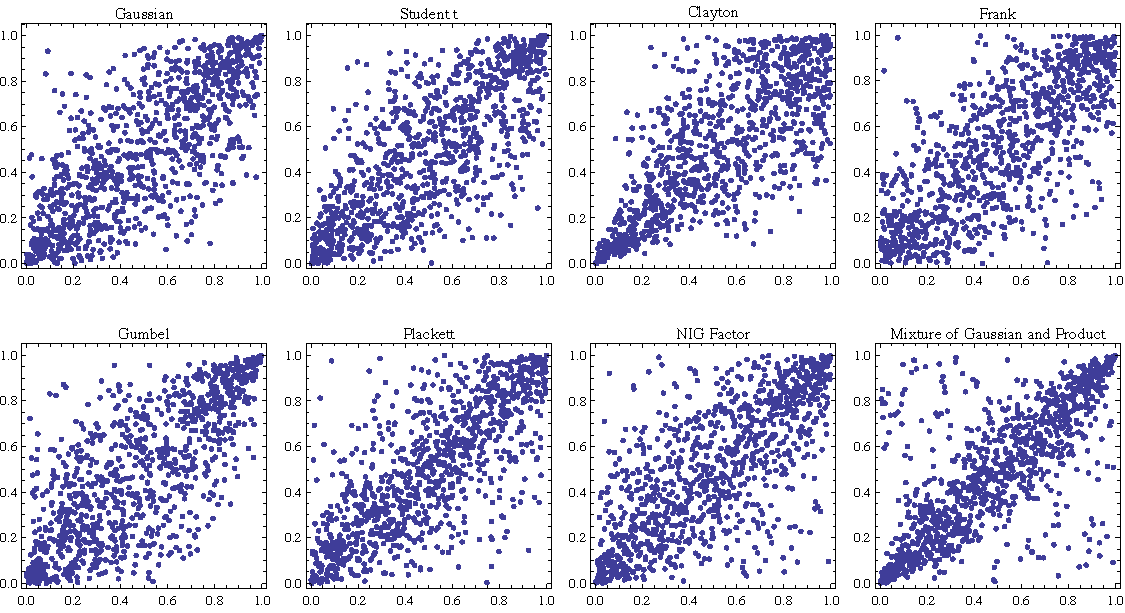
\includegraphics[width=\textwidth]{_pics/copulas_scatterplots.pdf}
  \caption{Scatterplots of samples drawn from various copulae. All
    copulae are calibrated to Spearman's $\rho$ of 0.75 before
    sampling.}\label{fig:copulaeScatterPlot} 
\end{figure}

As this hedging exercise concerns only portfolios with two assets, we
focus on the bivariate version of each copula. 

\subsection{Gaussian and $t$ Copulae}\label{sec:ellpitical-copulae}

The Gaussian and $t$ copulae are derived from Gaussian and $t$
distributions. 
The bivariate Gaussian copula is defined as
\begin{align*}
  \bm{C}(u,v) &= \Phi_{2, \rho}\{\Phi^{(-1)}(u), \Phi^{(-1)}(v)\} \nonumber \\
              &= \int_{-\infty}^{\Phi^{(-1)}(u)}
                \int_{-\infty}^{\Phi^{(-1)}(v)}
                \frac{1}{2\pi\sqrt{1-\rho^2}}
                \exp{\left\{
                \frac{s^2-2\rho st+t^2}{2(1-\rho^2)}
                \right\}} \dd s\, \dd t,\quad, u,v\in [0,1],
\end{align*}
where $\Phi_{2, \rho}$ is the bivariate Normal cdf
with zero mean, unit variance, with correlation coefficient $\rho$, and
$\Phi^{(-1)}$ is the quantile function of the univariate standard normal
distribution.
The Gaussian copula is fully specified by the correlation parameter $\rho$. \footnote{
The symbol $\rho$ is used to denote both the correlation parameter as
well as a general risk measure. However, it will be clear from the
context, what $\rho$ refers to.}
It has no tail dependence, which, in a finance context, implies that
it often underestimates tail risk.  

% The Gaussian copula density is
% \begin{equation*}
%   \bm{c}_\rho(u,v) = \frac{\bm{\varphi}_{2,\rho}\{\Phi^{(-1)}(u), \Phi^{(-1)}(v)\}}
%                      {\varphi\{\Phi^{(-1)}(u)\} \cdot \varphi\{\Phi^{(-1)}(v)\}} 
%                   = \frac{1}{2\pi\sqrt{1-\rho^2}}\exp\left\{
%                      -\frac{u^2 - 2\rho uv + v^2}{2(1-\rho^2)}
%                      \right\},
% \end{equation*}
% where $\bm{\varphi}_{2,\rho}(\cdot)$ is the pdf corresponding to
% $\Phi_{2, \rho}$, and $\varphi(\cdot)$ the standard normal
% pdf. \natp{\em [I think the abbreviations cdf and pdf where not
%   introduced. Please double-check.]}

Kendall's $\tau_K$ and Spearman's $\rho_S$ of the bivariate Gaussian copula are
    \begin{equation*}
        \tau_K(\rho) = \frac{2}{\pi}\arcsin\rho, \quad\quad
        \rho_S(\rho) = \frac{6}{\pi}\arcsin\frac{\rho}{2}.
        \end{equation*}

The $t$-copula has the form
\begin{multline*}
        \bm{C}(u,v) = \bm{T}_{2, \rho, \nu}\{T^{(-1)}_\nu(u), T^{(-1)}_\nu(v)\}\\
        = \int_{-\infty}^{T^{(-1)}_\nu(u)}
               \int_{-\infty}^{T^{(-1)}_\nu(v)}
            \frac{\Gamma\left(\frac{\nu+2}{2}\right)}
            {\Gamma\left(\frac{\nu}{2}\right)\pi\nu\sqrt{1-\rho^2}}
             \left(
        1+\frac{s^2-2st\rho+t^2}{\nu}
        \right)^{-\frac{\nu+2}{2}}\, \dd s\, \dd t,
    \end{multline*}
where $\bm{T}_{2, \rho, \nu}$ denotes the 
bivariate $t$ cdf with dependence parameter $\rho$ and degrees of
freedom parameter $\nu$, $\nu>2$,
and where $T^{(-1)}_\nu(\cdot)$ is the quantile function of a standard
$t$ distribution with parameter $\nu$. 

The $t$-copula and Gaussian copula with parameter $\rho$ have equal Kendall's $\tau$, \citep[see][and references therein]{demarta2005t}.
The $t$-copula has non-zero upper and lower tail dependence, which makes it more appropriate for dependence modelling in finance than the Gaussian copula.
% The copula density is
% \begin{align*}
%     \bm{c}(u,v) &= \frac{\bm{t}_{2, \rho, \nu}\{T^{(-1)}_\nu(u), T^{(-1)}_\nu(v)\}}
%     {t_\nu\{T^{(-1)}_\nu(u)\}\cdot t_\nu\{T^{(-1)}_\nu(v)\}},
%     \end{align*}
% where $\bm{t}_{2,\rho, \nu}$ is the pdf of $\bm{T}_{2, \rho, \nu}$
% and $t_\nu$ the density of standard $t$ distribution.

\subsection{Archimedean copulae}\label{sec:archimedean-copula}
The family of Archimedean copulae forms a large class of copulae with
many convenient features.
% Contrary to elliptical copulas, which are derived from
% elliptical distributions.
Archimedean copulas are determined via a simple parametric form of the
dependence structure. A prominent feature is the ability to model
asymmetric dependence structures.  

In general, an Archimedean copula takes the form
\begin{align*}
  \bm{C}_\theta(u,v) = \psi^{(-1)}\{\psi(u; \theta), \psi(v; \theta); \theta\},\quad u,v\in [0,1],
    \end{align*}
where $\psi:[0,1] \rightarrow [0,\infty)$ is a continuous, strictly
decreasing and convex function such that $\psi(1)=0$ for any
permissible dependence parameter $\theta$. The function $\psi$ is 
called the generator, with $\psi^{(-1)}$ its inverse.

The {\em Frank copula\/} (B3 in \citet{joe1997multivariate}) takes the form
\begin{align*}
    \bm{C}_{\theta}(u,v) &= \frac{1}{\theta}
    \log \left\{
    1 + \frac{(e^{-\theta u}-1)(e^{-\theta v}-1)}{e^{-\theta}-1}
    \right\}, \quad u,v\in [0,1],
    \end{align*}
    with $\theta \in [0, \infty]$ the dependence parameter. 
    It is a symmetric copula and cannot produce any tail
    dependence. The following parameters correspond perfect dependence
    and independence: $\bm{C}_{-\infty} = \bm{M}$, $\bm{C}_1 = \bm{\Pi}$,
    and $\bm{C}_\infty = \bm{W}$. 
    % The copula density is
    % \begin{align*}
    %   \bm{c}_{\theta}(u,v)
    %   &= \frac{\theta e^{\theta(u+v)(e^\theta-1)}}
    %     {\left\{e^\theta-e^{\theta u}-e^{\theta v}+e^{\theta (u+v)}\right\}^2}.
    % \end{align*}
    The Frank copula has Kendall's $\tau$ :
\begin{align*}
    \tau_K(\theta) = 1-4\frac{D_1\{-\log(\theta)\}}{\log(\theta)},
    \end{align*}
% and
% \begin{align*}
%     \rho_S(\theta) = 1-12\frac{D_2\{-\log(\theta)\} - D_1\{\log(\theta)\}}{\log(\theta)},
%     \end{align*}
where $D_1$ and $D_2$ are the Debye function of order 1 and 2, with
the Debye function defined as $D_n =
\frac{n}{x^n}\int_0^x\frac{t^n}{e^t-1}dt$.
We refer readers to \citet[p.998]{abramowitz1972handbook} for definition of the Debye function. 

The {\em Gumbel copula\/} (B6 in \citet{joe1997multivariate}) has
distribution function
\begin{equation*}
  \bm{C}_{\theta}(u,v) = \exp{-\{ (-\log(u))^\theta +(-\log(v))^\theta 
    \}^{\frac{1}{\theta}}},
\end{equation*}
where $\theta \in [1,\infty)$ is the dependence parameter.
Its  Kendall's tau takes the form \begin{equation*}
  \tau_K(\theta) =\frac{\theta-1}{\theta}. 
 \end{equation*}
It has upper tail dependence with dependence parameter $\lambda^U
= 2-2^{\frac{1}{\theta}}$ and displays no lower tail dependence. 
    
While the Gumbel copula cannot model perfect counter-dependence
\citep{Nelsen2002}, $\bm{C}_{1} = \bm{\Pi}$ models independence, 
and $\lim_{\theta\rightarrow\infty} \bm{C}_\theta = \bm{W}$ models
perfect dependence. 


The {\em Clayton copula\/} takes the form
\begin{equation*}
  \bm{C}_{\theta}(u,v) = \left\{
    \max(u^{-\theta}+v^{-\theta}-1,0)\right\}^{-\frac{1}{\theta}},
\end{equation*}
where $\theta \in (-\infty, \infty)$ is the dependence parameter.
The Clayton copula, by contrast to Gumbel copula,
generates lower tail dependence with $\lambda^L =
2^{-\frac{1}{\theta}}$, but cannot generate upper tail dependence.
Moreover, $\lim_{\theta\rightarrow -\infty} \bm{C}_\theta = \bm{M}$, $\bm{C}_0 =
\bm{\Pi}$, and $\lim_{\theta\rightarrow\infty} \bm{C}_\theta = \bm{W}$. 
Kendall's $\tau$ of the Clayton copula is given by 
\begin{align*}
    \tau_K(\theta) =\frac{\theta}{\theta+2}.
    \end{align*}

\subsection{Mixture Copula}\label{sec:mixture-copula}
The mixture copula is a linear combination of copulae. 
The distribution of a 2-dimensional random variable
$\bm{X}=(X_1,X_2)^\top$ is written as linear combination of $K$
copulae 
\begin{equation*} 
    \bm{C}(u,v)= \sum_{k=1}^K p^{(k)} \cdot \bm{C}^{(k)}\{F^{(-1)}_{X_1}(u),
    F^{(-1)}_{X_2}(v); \bm{\theta^{(k)}}\}, \quad u,v\in [0,1].
  \end{equation*}
  Here, $\bm{\theta^{(k)}}$ refers to the parameters of the
    $k$-th copula.
%     Likewise, the copula density is a linear
%     combination of copula densities 
% \begin{align*}
%     \bm{c}(u,v)= \sum_{k=1}^K p^{(k)} \cdot \bm{c}^{(k)}\{F^{(-1)}_{X_1}(u),
%     F^{(-1)}_{X_2}(v); \bm{\theta^{(k)}}\}.
%     \end{align*}
   
While Kendall's $\tau$ of the mixture copula is not known in closed form,
Spearman's $\rho$ is easily derived as 
\begin{equation*}
  \rho_S = \sum_{k=1}^K p^{(k)} \cdot \rho_S^{(k)}. 
\end{equation*}

% \natp{\em [Old text below.]}

% While Kendall's $\tau$ of the mixture copula is not known in closed form,
% Spearman's $\rho$ is specified by the following statement. 
% \begin{proposition}
%   Let $\rho_S^{(k)}$ be Spearman's $\rho$ of the $k$-th component
%   Spearman's $\rho$ of the mixture copula is given by 
%   \begin{align*}
%         \rho_S = \sum_{k=1}^K p^{(k)} \cdot \rho_S^{(k)}.
%         \end{align*}
%     \end{proposition}

% \begin{proof}
%   Since Spearman's $\rho$ is defined as \citep{Nelsen1999}
%   \begin{equation*}
%     \rho_S = 12 \int_{\mathbb{I}^2} \bm{C}(s,t) ds dt - 3,
%   \end{equation*}
%   Spearman's $\rho$ of the the mixture copula is given by summation
%   of the components 
%   \begin{align*}
%     \rho_S = 12 \int_{\mathbb{I}^2} \sum_{k=1}^K p^{(k)} \cdot
%     \bm{C}^{(k)}(s,t) ds dt - 3. 
%   \end{align*}
% \end{proof}
% \natp{\em [Continue here.]}

An example of a mixture copula is the Fr\'echet class of copulae, which
are given by convex combinations of $\bm{W}$, $\bm{\Pi}$, and $\bm{M}$
\citep{Nelsen1999}.  

We use the {\em Gaussian Mix Independent Copula (GMI)} in our analysis,
i.e., 
\begin{equation*}
  \bm{C}(u,v) = p\, \bm{C}^\text{Gaussian}_\theta (u,v) + (1-p)(uv),\quad p\in [0,1].
\end{equation*}
% with corresponding density 
% \begin{equation*}
%   \bm{c}(u,v) = p\, \bm{c}^\text{Gaussian}(u,v) + (1-p).
% \end{equation*}

This mixture models the amount of ``random noise'' that appears in the
off-diagonal region of the dependence structure where the Gaussian copula has no control.
In the hedging exercise, the structure of the off-diagonal ``random noise'' is not our main concern, 
but the amount of it might affect the hedging effectiveness.

\subsection{NIG factor copula}

Normal Inverse Gaussian (NIG) distribution is a flexible and yet analytical tractable distribution introduced by
\citep{BarndorffNielsen1997}.
The {\em NIG factor copula} is constructed based on the characteristics of the NIG disribution. 
This section presents the version of NIG factor copula we use in this work.
The NIG distribution has density function
\begin{equation*}
  g(x; \alpha,\beta, \mu, \delta) = \frac{\alpha}{\pi} \e^{\delta
    \sqrt{\alpha^2-\beta^2} -\beta\mu} \frac{1}{q((x-\mu)/\delta)}
  K_1\left[\delta \alpha q\left(\frac{x-\mu}{\delta}\right) \right]
  \e^{\beta x},\quad x>0,
\end{equation*}
where $q(x) = \sqrt{1+x^2}$ and where $K_1$ is the modified Bessel
function of third order and index $1$. The parameters satisfy $0\leq
|\beta|\leq \alpha$, $\mu\in \R$ and $\delta>0$, and have
the following interpretation: $\mu$ and $\delta$ are location and
scale parameters, respectively, $\alpha$ determines the heaviness of
the tails and $\beta$ determines the degree of asymmetry. If
$\beta=0$, then the distribution is symmetric around $\mu$.

The cdf and quantile function of NIG distribution, denoted by $G(x; \alpha, \beta, \mu, \delta)$ and $G^{(-1)}(x; \alpha, \beta, \mu, \delta)$,
 have no known analytical form.
 In this work, they are computed via numerical integration of the density and by simulation.

The NIG distribution belongs to
the class of so-called {\em normal
variance-mean mixture distributions},  (see Section 3.2 of 
\citet{McNeil2005}): $X$ follows an
$\text{NIG}(\alpha,\beta,\mu,\delta)$ distribution if $X$ conditional
on $W$ follows a normal distribution with mean $\mu+\beta W$ and
variance $W$, i.e., 
\begin{equation*}
  X|W\stackrel{\mathcal L}\sim \Ncdf(\mu + \beta W, W),
\end{equation*}
where $W$ follows an {\em inverse Gaussian distribution}, denoted by
$\text{IG}(\delta, \sqrt{\alpha^2-\beta^2})$.

The simulation procedure of the NIG$(\alpha, \beta, \mu, \delta)$
distribution is a natural result of the above decomposition.  
To simulate the NIG distribution, first simulate a random variable $w \sim IG(\delta, \sqrt{\alpha^2-\beta^2})$, 
then simulate $x \sim N(\mu+ \beta w, w|w)$. 

The moment-generating function of the NIG distribution is given by
\begin{equation*}
  M(u; \alpha, \beta, \mu, \delta) = \exp\left( \delta
    \left(\sqrt{\alpha^2-\beta^2} - \sqrt{\alpha^2 - (\beta +
        u)^2}\right) + \mu u\right). 
\end{equation*}
As a direct consequence, moments are easily calculated with the
expectation and variance of the NIG distribution being
\begin{align*}
  \mathbb E X &= \mu +
                \frac{\delta \beta}{\sqrt{\alpha^2-\beta^2}}
  \end{align*}
\begin{align} \label{eq:5}
  \text{Var}(X) &= \frac{\alpha^2\delta}{(\alpha^2-\beta^2)^{3/2}}.
\end{align}

It is easily seen from the moment-generating function that the NIG distribution is preserved under linear combinations, provided
the variables share the parameters $\alpha$ and $\beta$. 
\begin{prop}
  \label{prop:NIG}
  Let $Z\sim \text{NIG}(\alpha, \beta, \mu, \delta)$ and
  $Z_i\sim \text{NIG}(\alpha, \beta, \mu_i, \delta_i)$,
  $i=1,\ldots, n$ be independent NIG-distributed random
  variables. Then:
  \begin{enumerate}
  \item  $X_i = Z + Z_i\sim \text{NIG}(\alpha,\beta,\mu+\mu_i,
  \delta+\delta_i)$,
\item and 
  \begin{align}
    \text{Cov}(X_i,X_j) &= \text{Var(Z)},\nonumber\\
    \text{Corr}(X_i,X_j) &= \frac{\delta}{\sqrt{(\delta+\delta_i)
                           (\delta+\delta_j)}}. \label{eq:6}
  \end{align}
\end{enumerate}
\end{prop}
\begin{proof}
  \begin{enumerate}
  \item This follows directly from the moment-generating function. 
  \item For the covariance,
    \begin{equation*}
      \text{Cov}(X_i,X_j)
      = \E[(Z+Z_i) (Z+Z_j)] - \E[Z+Z_i] \E[Z+Z_j]
      = \E[Z^2] -(\E Z)^2.
    \end{equation*}
    The correlation is determined directly from \ref{eq:5}.
  \end{enumerate}
\end{proof}

The NIG distribution is popular in many areas of
financial modelling; for example, it gives rise 
to the normal inverse Gaussian L\'evy process, which may be represented
as a Brownian motion with a time change.
In the setting here, we consider the {\em NIG factor copula}, which is
not directly derived from the multivariate NIG distribution, but
determined through a factor structure instead. \footnote{The factor structure,
which was applied e.g.\ in \citep{Kalemanova2007} for calibrating CDO's,
gives additional flexibility as it does not force the components to
have a mixing variable $W$.}

The bivariate NIG factor model is given by
\begin{align*}
  X &= Z + Z_1 \\ 
  Y &= Z + Z_2,
  \end{align*}
where $Z \sim \text{NIG}(\alpha, \beta, \mu, \delta)$, $Z_1 \sim \text{NIG}(\alpha, \beta, \mu_1, \delta_1)$, 
$Z_2 \sim \text{NIG}(\alpha, \beta, \mu_2, \delta_2)$, and $Z, Z_1, Z_2$ are mutually independent. 

The following normalising steps reduce the number of parameters to three:
\begin{enumerate}
  \item Set $\mu = \mu_1= \mu_2 = 0$ . The location parameter does not affect the correlation structure.
  \item Set $\delta_1 = \delta_2 = \frac{(\alpha^2-\beta^2)^{3/2}}{\alpha^2}$ such that $Z_1$ and $Z_2$ are unit variance. 
  Normalising the scale parameter does not affect the correlation structure.
\end{enumerate}
  % Denote the margins by $u,v \sim U(0,1)$. 
% The NIG factor model is obtained by transforming the unifrom margins to standardised NIG distriutions.
The dependence between $X$ and $Y$ is now fully captured by $\alpha, \beta$, and $\delta$.  

% 
% \natp{\em [Can you provide a reference for the Proposition?]}
\begin{prop}
  Let $u,v \in [0,1]$,
  $\alpha, \beta \in \mathbb{R}$ satisfying $0 \leq |\beta| \leq \alpha$, $\delta >0 $,
  $f(\cdot) = g\left(\cdot; \alpha, \beta, 0, \delta \right)$, 
  and $F (\cdot) = G\left(\cdot; \alpha, \beta, 0, \frac{(\alpha^2-\beta^2)^{3/2}}{\alpha^2}\right)$.
  The {\em NIG factor copula} is 
  \begin{equation*}
    C(u,v) = \int_\mathbb{R} F\left\{F^{(-1)}(u)-z\right\}
    F\left\{F^{(-1)}(v)-z\right\}f(z)dz.
  \end{equation*}

\end{prop}

\begin{proof}
  Let $F_X$ and $F_Y$ be the cdfs, $F_X^{(-1)}$ and $F_Y^{(-1)}$ be the quantile functions of $X$ and $Y$ respectively. 
  \begin{align*}
    C(u,v) &= \p\left(F_X(X) \leq u, F_Y(Y)\leq v\right)\\
           &= \E \left\{\left.\p\left(F_X(X) \leq u, F_Y(Y)\leq v \right|Z\right)\right\}\\
           &= \E \left\{\left.\p\left(Z_1 \leq F_X^{(-1)}(u)-Z, Z_2 \leq F_Y^{(-1)}(v)-Z \right|Z\right)\right\}\\
           &=  \int_\mathbb{R} F\left\{F^{(-1)}(u)-z\right\}F\left\{F^{(-1)}(v)-z\right\}f(z)dz.
  \end{align*} 
\end{proof}

% The parameters $\alpha, \beta, \tilde \delta$ fully control the dependence between $u$ and $v$, $u, v \sim U(0,1)$, captured by the NIG factor copula.
We refer readers to \citet{krupskii2018factor} for the methodology of constructing factor copulae. 
See also \citet[Section 3.10]{joe2014dependence} and \citet{krupskii2013factor}. 

The quantile dependence and Spearman's rho of NIG factor copula have no known analystical form.
In this work, the quantile dependence is computed numerically; 
Spearman's rho is approximated by Spearman's rho of the bivariate Gaussian copula. 
When $\beta \rightarrow 0$ and $\alpha \rightarrow \infty$, the NIG
distribution behaves similarly to the Gaussian distribution, 
making the (bivariate) NIG factor copula behave similarly to the
(bivariate) Gaussian copula. 
Therefore, the NIG factor copula's Spearman's rho is well approximated by the Spearman's rho of the bivariate Gaussian copula.


% \natp{\em [Please clarify that $\circ$ refers to composition. Clean
%   up notation, e.g.\ marginals can be denoted $F_F$ and $F_S$, Use
%   just $C$ for the copula. What are $Z_1$ and $Z_2$? I don't find the
%   formula in the paper mentioned. Also, where is the formula for
%   Kendall's tau taken from?]}
%  The NIG factor copula is obtained by transforming the margins to
% uniforms (see Sklar's Theorem), giving (e.g.\
% \citep{krupskii2013factor}):
% \begin{equation*}
%   C_{r^S, r^F}(F_{r^S}(r^S), F_{r^F}(r^F)) = \int_\mathbb{R}
%   F_{Z_1}(F_{X_1}^{(-1)} \circ F_{r^S}(r^S) -z) \cdot
%   F_{Z_2}(F_{X_2}^{(-1)} \circ F_{r^F}(r^F) -z) \cdot
%   f_Z(z) dz.
%   \end{equation*}
% If the margins are continuous, then Spearman's rho of NIG factor
% copula is 
% \begin{equation*}
%   \rho_S = 12 \int \int \int_{\mathbb{R}^3}
%   F_{X_1}(x_1) \cdot
%   F_{X_2}(x_2) \cdot
%   f_{Z_1}(x_1-z) \cdot
%   f_{Z_2}(x_2-z) \cdot
%   f_Z(z) dx_1 dx_2 dz - \frac{1}{48}.x
%   \end{equation*}

% \begin{proof}
%   \begin{align}
%   \rho_S(r^S, r^F) &= \rho\{F_{r^S}(r^S), F_{r^F}(r^F)\} \\
%     &= \rho\{F_{X_1}(X_1), F_{X_2}(X_2)\} \\
%     &= 12 \cdot \mathbb{E}\{F_{X_1}(X_1) \cdot F_{X_2}(X_2) \} - \frac{1}{48}\\
%     &= 12 \cdot \int \int_{\mathbb{R}^2} F_{X_1}(X_1) \cdot F_{X_2}(X_2) dF_{X_1,X_2}(x_1,x_2)\\
%     \end{align}
%   Because
%   \begin{align}
%     F_{X_1,X_2}(x_1,x_2) &= \mathbb{P}(X_1 \leq x_1, X_2 \leq x_2)\\
%     &= \mathbb{P}(Z_1 \leq x_1 - Z, Z_2 \leq x_2 - Z) \\
%     &= \int_\mathbb{R}\mathbb{P}(Z_1 \leq x_1 - z) \cdot \mathbb{P}(Z_2 \leq x_2 - z) \cdot f_Z(z) dz,
%     \end{align}
%   so,
%   \begin{align}
%     \rho_S(r^S, r^F) = 12 \cdot \int \int \int_{\mathbb{R}^3} F_{X_1}(x_1) \cdot F_{X_2}(x_2) \cdot f_{Z_1}(x_1 -z) \cdot f_{Z_2}(x_2 -z) \cdot f_{Z}(z) dx_1 dx_2 dz -\frac{1}{48}
%     \end{align}
%   \end{proof}


\subsection{Plackett copula}\label{subsec:other-copula}
The Plackett copula has distribution function
\begin{align*}
    \bm{C}_{\theta}(u,v) &= \frac{1+(\theta-1)(u+v)}{2(\theta-1)}
                         - \frac{\sqrt{\{
    1+(\theta-1)(u+v)\}^2 - 4uv\theta(\theta-1)}}{2(\theta-1)},
\end{align*} where $0 \leq \theta < \infty$.
Spearman's rho is given by 
\begin{align*}
    \rho_S(\theta) = \frac{\theta+1}{\theta-1} - \frac{2\theta \log
  \theta}{(\theta-1)^2}. 
    \end{align*}

The Placket copula possesses a special property:
the cross-product ratio is equal to the dependence parameter
\begin{equation} \label{eq:PlackettCrossProduct}
    % &\phantom{=}
    \frac{\p(U \leq u, V \leq v) \cdot \p(U > u, V > v)}
    {\p(U \leq u, V > v) \cdot \p(U > u, V \leq v)}\nonumber
    =
      \frac{\bm{C}_\theta(u,v)\{1-u-v+\bm{C}_\theta(u,v)\}}{\{u-\bm{C}_\theta(u,v)\}\{v-\bm{C}_\theta(u,v)}\nonumber 
    = \theta.
\end{equation}
In words, the dependence parameter is equal to the ratio of the 
number of concordance pairs and the number of discordance pairs of a 
bivariate random variable. 

\subsection{Calibration}\label{sec:estimation}
We trace back the usage of method of moments (MM) to calibrate copulae to \citet{Genest1987, genest1993statistical} 
where the moments mainly refer to Kendall's tau $\tau_K$ or Spearman's rho $\rho_S$.
Adapted from \cite{oh2013simulated}, we extend MM to quantile dependence measures. 
Quantile dependence is denoted by $\lambda_q$ for quantile level $q$.

Spearman's rho, Kendall's tau, and quantile dependence of the copula $C$ are defined as
\begin{align*}
  \rho_S &= 12 \int\int_{I^2} C_{\bm{\theta}}(u,v)\, \dd u\, \dd v-3\label{eq:rho_S}\\
  \tau_K &= 4\E[C_{\bm{\theta}}\{F_X(x), F_Y(y)\}]-1,\\
  \lambda_q &=
  \begin{cases}
    \p(F_X(X)\leq q| F_Y(Y)\leq q) = \displaystyle \frac{C_{\bm{\theta}}(q,q)}{q},
    &\text{ if } q\in (0,0.5],\\
    \p(F_X(X)>q|F_Y(Y)>q) =\displaystyle \frac{1-2q+C_{\bm{\theta}}(q,q)} {1-q},
    &\text{ if } q\in (0.5,1).
  \end{cases}
\end{align*}
The empirical counterparts are
\begin{align*}
  \hat\rho_S &= \frac{12}{n} \sum_{k=1}^n \hat F_X(x_k) \hat F_Y(y_k)
               -3,\\
  \hat\tau_K &= \frac{4}{n}\sum_{k=1}^n \hat{C}\{\hat{F}_X(x_i),\hat{F}_X(y_i)\} -1 ,\\
  \hat\lambda_q &=
                  \begin{cases}
                    \displaystyle\frac{1}{n} \sum_{k=1}^n \frac{\1_{\{\hat
                        F_X(x_k)\leq q, \hat F_Y(y_k)\leq q\}}} {q},
                    &\text { if } q\in (0, 0.5],\\
                    \displaystyle \frac{1}{n} \sum_{k=1}^n
                    \frac{\1_{\{\hat F_X(x_k)>q, \hat F_Y(y_k)>q\}}}
                    {1-q}, &\text { if } q\in (0.5,1),
                  \end{cases}
\end{align*}
where $\displaystyle \hat{F}(x) =
  \frac{1}{n}\sum_{k=1}^n 1_{\{x_i\leq x\}}$ and
$\displaystyle \hat{C}(u,v) = \frac{1}{n}\sum_{k=1}^n 1_{\{u_i\leq u, v_i\leq v\}}$. 

Denote by $\bm{m}(\bm{\theta})$ the $m$-dimensional vector of
dependence measures according the dependence parameters
$\bm{\theta}$,and let $\hat{\bm{m}}$ be the corresponding empirical
counterpart. 
The difference between dependence measures and their counterpart is denoted by
\begin{equation*}
    \bm{g}(\bm{\theta}) = \hat{\bm{m}} - \bm{m}(\bm{\theta}),
\end{equation*}
and the {\em MM estimator} is
\begin{equation*}
    \hat{\bm{\theta}} = \argmin_{\bm{\theta}\in \bm{\Theta}} \bm{g}(\bm{\theta})^\top
    \hat{\bm{W}}
     \bm{g}(\bm{\theta}),
\end{equation*}
where $\hat{W}$ is a positive definite weight matrix.
In this work, we use
$\bm{m}(\bm{\theta}) = (\rho_S, \lambda_{0.05}, \lambda_{0.1}, 
\lambda_{0.9}, \lambda_{0.95})^\top$
for calibration with 
$\hat{W}$ set to the identity matrix. 
We replace Spearman's rho by Kendall's tau when the analytical form of the former is not available. 

While maximum likelihood estimation is a viable procedure to calibrate copula, 
we choose MM as the estimation procedure in this work. 
Figure~\ref{fig:quantile dependence1} shows the empirical quantile
dependence of Bitcoin and CME futures and the copula implied quantile
dependence of the MLE and MM calibration procedures. 
Although the MLE is a better fit to a range of quantile dependence in
the middle, it fails to address the situation in the tails. 

\begin{figure}[h]
%\includegraphics[width=\textwidth]{_pics/t Copula quantile dependence.png}
\includegraphics[width=\textwidth]{_pics/Gumbel Copula quantile dependence.pdf}
\includegraphics[width=\textwidth]{_pics/Clayton Copula quantile dependence.pdf}
  \caption{Quantile dependences of Gumbel and Clayton copulas. The
    \textcolor{darkblue}{blue circle dots} are the quantile dependence
    estimates of Bitcoin and CME future, the \textcolor{darkblue}{blue
      dashed lines} are the estimates' 90\% confidence interval. 
  The \textcolor{orange}{orange dotted line} is the copula implied
  quantile dependence by MM estimation. The
  \textcolor{lightblue}{light blue dotted line} is the copula implied
  quantile dependence by MLE estimation.  
  \href{https://github.com/QuantLet/Hedging-Cryptos-with-Bitcoin-Futures/blob/main/newToQuantlet/Pynotebooks/figures/figure 2.ipynb}{\includegraphics[height=\baselineskip]{_pics/qletlogo_tr.png}}}
  
\label{fig:quantile dependence1}
\end{figure}

\subsection{Copula selection}\label{subsec:copula-selection}
As the dependence structure of price data changes
across time, we allow for a flexible choice of the best-fitting
copula, by re-calibrating periodically and re-evaluating performance
of the various copulas. 
In each re-calibration, we select the best-fitting
copula, characterised by the lowest {\em Akaike Information Criterion
  (AIC)},
\begin{equation*}
 \text{AIC} = 2k- 2 \log(L),
\end{equation*}
where $k$ is the number of estimated
parameters and $L$ is the likelihood \citep{Akaike1973}. 

% they tend to suggest the same copula as the best fitting one.
%Simulation studies has also been carried out to compare different copula selection methods, see \cite{}.
Other model selection criteria, such as the TIC~\citep{takeuchi1976distribution} or likelihood ratio test could be used instead.
For a survey of model selection and inference, see \cite{anderson1998comparison}.
Among various copula selection procedures, AIC is a popular choice for
its applicability, see e.g. \cite{breymann2003dependence}.
In our case, the AICs are calculated only with dependence likelihood
since the marginals are modelled via kernel density estimators.
The selected copula will then enter the calculation of the optimal
hedge ratio.
% We consider the copula with the lowest AIC for a particular set of data the best fitting one and use it to generate OHR.

\section{Risk measures}\label{subsec:spectral-risk-measures}
The optimal hedge ratio is determined for the following variety of risk measures: variance, Value-at-Risk (VaR), Expected Shortfall (ES), and Exponential Risk Measure (ERM).
A summary of risk measures being used in portfolio selection problem
can be found in \citet{hardle2008applied}. 
The risk measures here serve as risk minimization objectives, i.e. loss functions for searching the optimal hedge ratio. 
%They are used in many literature about hedging, e.g. ;
%The risk measures are also used by regulatory bodies,
%for example Basel III ....

The risk measures are defined as follows.
Let $Z$ be a random
variable with distribution function $F_Z$.
\begin{enumerate}
\item Variance: $\text{Var}(Z) = \E[(Z-\E Z)^2]$. 
\item VaR at confidence level $\alpha$: $\text{VaR}_\alpha(Z) = -F_{Z}^{(-1)}(1-\alpha)$
\item ES at confidence level $\alpha$: $\text{ES}_\alpha(F_Z) = -\frac{1}{1-\alpha}\int_0^{1-\alpha}F_Z^{(-1)}(p)\dd p$
\item ERM with Arrow-Pratt coefficient of absolute risk
  aversion $k$:
  \begin{equation*}
    \text{ERM}_k(Z) = -\int_{[0,1]}\phi(p) F_Z^{(-1)}(p)\dd p,
  \end{equation*}
  where $\phi$ is a weight function described in (\ref{eq:phi}) below.
\end{enumerate}

VaR, ES, and ERM fall into the class of spectral risk measures (SRM),
which have the form \citep{Acerbi2002}%, adam2008spectral,dowd2008spectral}
\begin{equation*}
  \rho_\phi(Z) = - \int_0^1 \phi(p) F_{Z}^{(-1)}(p)\dd p,
\end{equation*}
where $p$ is the loss quantile and $\phi(p)$ is a user-defined
weighting function defined on $[0,1]$.
We consider only so-called admissible risk spectra $\phi(p)$, i.e.,
fulfilling %(named by \citet{Acerbi2002})
\begin{enumerate}[label=(\roman*)]
\item $\phi$ is positive,
\item $\phi$ is decreasing,
\item and $\int_{[0,1]}\phi(p)\dd p=1$. 
\end{enumerate}

The VaR's $\phi(p)$ gives all its weight on the $1-\alpha$ quantile of
$Z$ and zero elsewhere, i.e., the weighting function is a Dirac delta
function, and hence it violates the (ii) property of admissible risk
spectra.  
The ES' $\phi(p)$ gives all tail quantiles the same weight of
$\displaystyle\frac{1}{1-\alpha}$ and non-tail quantiles zero weight. 
The ERM assumes investors' risk preference are in the form of an
exponential utility function $U(x)=1-e^{kx}$, so its corresponding
risk spectrum is defined as
\begin{equation*}
  \phi(p) =\frac{k e^{-k(1-p)}}{1-e^{-k}} , \label{eq:phi}
\end{equation*}
where $k$ is the Arrow-Pratt coefficient of absolute risk aversion. 
The parameter $k$ has an economic interpretation as being the ratio
between the second derivative and first derivative 
of investor's utility function on an risky asset,
\begin{equation*}
  k = -\frac{U''(x)}{U'(x)},
\end{equation*}
for $x$ in all possible outcomes.
In case of the exponential utility, $k$ is the the constant absolute risk aversion (CARA).

